\documentclass[%
thesis=student,% bachlor's or master's thesis
coverpage=false,% do not print an extra cover page
titlepage=false,% do not print an extra title page
headmarks=true, % headmarks can be switched on or off
twoside=false,
english,% or `english`
font=libertine, % use `libertine` font; alternatives: `helvet` / `palatino` / `times`
math=newpxtx, % math font `newpxtx`; alternatives: `ams`, `pxtx`
BCOR=5mm,% binding correction - adapt accordingly
coverBCOR=11mm,% binding correction for the cover - adapt accordingly
]{tumbook}

\makeatletter %redefine some labels from the TUM template
\setbool{@twoside}{false}
\provideName{\@tum@examiner@}{Supervisor}{Themensteller} % or `Themenstellerin`
\provideName{\@tum@supervisor@}{Advisor}{Betreuer} % or `Advisor` / `Betreuerin`
\makeatother

%\usepackage{subfig}
\usepackage{scrhack}
%\usepackage{lmodern}
\usepackage{anyfontsize}
\usepackage{booktabs}% for more beautiful tables
\usepackage{cleveref}% intelligent references
\usepackage{diffcoeff}
\usepackage{amsmath}
\usepackage{physics}
\usepackage{graphicx}
\usepackage{bbm}
\graphicspath{{figures/}}
\usepackage{pgfplots}
\pgfplotsset{compat=1.18}
\usepackage{float}
\usepackage{tikz}
\usetikzlibrary{shapes}
\usetikzlibrary{shapes.misc}
\usepackage{dsfont}
\usepgfplotslibrary{colorbrewer}
%Literatur
\usepackage[%
    backend=bibtex, %, or `biber` on more up-to-date systems
    sortcites, % sort automatically
    sorting=none, % sort order
    safeinputenc, % solves problems with unicode-formatted author names etc.
    citestyle=numeric, %
    bibstyle=numeric, %
    hyperref=true, % provide clickable links
    maxbibnames=4, % shorten author list for more than 4 names
    maxcitenames=4, % use at most 4 names for key
    url=false, % do not print URLs
    doi=false, % do not print DOIs
    giveninits=true,
    ]%
{biblatex}
\addbibresource{literature.bib}

% automatische Anführungszeichen
\usepackage[autostyle=true]{csquotes}

\title{Benchmarking a Tensor Network Algorithm for the HOPS-Method to Simulate Open non-Markovian Quantum Sytems}

\author{Benjamin Sappler}

\degree{Bachlor of Science}% or `Bachlor of Science`
\dateSubmitted{June 15, 2023}% preferably use some universally recognized date format

\examiner{Prof.$\,$Dr.$\,$Christian Mendl}% `Themensteller`
\supervisor{Richard Milbradt}% `Betreuer`

\begin{document}

\begin{center}
    \thispagestyle{empty}
    \theTUMLogo[height=2.5cm, color=TUMBlue]
    \vspace*{0.5cm}
    \par\textsc{\Huge Technical University of Munich}
    \vspace*{0.5cm}
    \par\textsc{\Large School of Computation, Information and Technology}
    \vspace*{0.3cm}
    \par\textsc{\Large Department of Computer Science}
    \vspace*{2cm}
    \par\Large Bachelor's Thesis in Informatics
    \vspace*{1.5cm}
    \par\textbf{\Huge Benchmarking a Tensor Network Algorithm for the HOPS-Method to Simulate Open non-Markovian Quantum Sytems}
    \vspace*{1.5cm}
    \par\Large Benjamin Sappler
    \vfill
    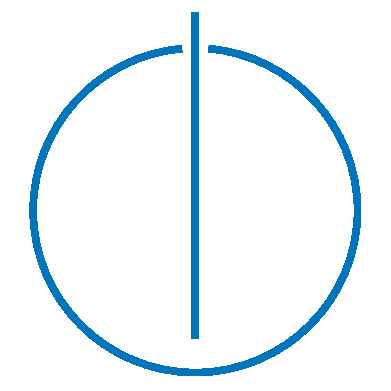
\includegraphics[width=2.5cm]{TUM_IN_Logo.pdf}
    \vfill
\end{center}

\newpage

\begin{center}
    \thispagestyle{empty}
    \theTUMLogo[height=2.5cm, color=TUMBlue]
    \vspace*{0.5cm}
    \par\textsc{\Huge Technical University of Munich}
    \vspace*{0.5cm}
    \par\textsc{\Large School of Computation, Information and Technology}
    \vspace*{0.3cm}
    \par\textsc{\Large Department of Computer Science}
    \vspace*{2cm}
    \par\Large Bachelor's Thesis in Informatics
    \vspace*{1.5cm}
    \par\textbf{\Huge Benchmarking a Tensor Network Algorithm for the HOPS-Method to Simulate Open non-Markovian Quantum Sytems}
    \vspace*{1.5cm}
    \par\textbf{\Huge Benchmarking eines Tensor Network Algorithmus für die HOPS-Methode zur Simulation offener, nicht-Markovianischer Quantensysteme}
    \vspace*{2cm}
    \par
    \begin{tabular}{l l}
        Author: & Benjamin Sappler\\
        Supervisor: & Prof. Dr. Christian Mendl\\
        Advisor: & Richard Milbradt, M.Sc.\\
        Submitted: & Munich, June 15, 2023\\
    \end{tabular}
\end{center}

\newpage

\thispagestyle{empty}
\null\vfill
\@tum@student@disclamer@block@

\begin{refsection}
\thispagestyle{empty}

\newpage

\thispagestyle{empty}

\section*{Abstract}
The dynamics of open quantum systems is of great interest for many fields in physics and chemistry. For systems strongly interacting
with their environments the dynamics are inherently non-Markovian, which is notoriously difficult to study and simulate.
In this thesis I implement in detail the Hierarchy of Pure States (HOPS) \cite{Suess:2014} and the recently developed Hierarchy of Matrix Product States (HOMPS) \cite{Gao:2022} methods,
which can be used to simulate non-Markovian dynamics. I then benchmark both methods using the spin-boson model.

\section*{Zusammenfassung}
Die Dynamik offener Quantensysteme ist in vielen Bereichen der Physik und Chemie von großer Bedeutung. Systeme, die stark mit ihrer Umgebung interagieren,
besitzen eine inherent nicht-Markovianische Dynamik, was erhebliche Probleme bei der theoretischen Beschreibung und Simulation dieser Systeme verursachen kann.
In dieser Arbeit implementiere ich die Hierarchy of Pure States (HOPS) \cite{Suess:2014} und die Hierarchy of Matrix Product States (HOMPS) \cite{Gao:2022}
Methoden, die für die Simulation offener, nicht-Markovianischer Systeme benutzt werden können. Anschließend benchmarke ich beide Methoden mit dem Spin-Boson Modell. 

\newpage

\tableofcontents
\thispagestyle{empty}

\mainmatter{}

\chapter{Introduction}
\label{chap:Introduction}
Open quantum systems, ie. quantum systems that are interacting with an environment, are important for modelling many complex
processes, like the decoherence of quantum computers and processes in the field of chemical physics.
Most of the time, these systems cannot be described analytically, but only numerically. Thus, the field of open quantum system
simulation is very important.\\
A popular approach for the simulation of open quantum systems is the Hierarchy Of Pure States (HOPS) \cite{Suess:2014}.
With HOPS, one can integrate the non-Markovian quantum state diffusion equation and simulate non-markovian open quantum systems.
Recently, it was shown that the popular Matrix Product State formalism can be used to derive a Hierarchy Of Matrix Pure States (HOMPS),
which can drastically improve the memory requirements for HOPS. \\
The goal of this thesis is to implement and benchmark both HOPS and HOMPS in detail. I start by giving a derivation of HOPS
from the non-markovian quantum state diffusion equation in section \ref{chap:HOPS}. Next, I explain in detail how HOPS can be implemented and
test the method on the spin boson model in section \ref{chap:Implementing_HOMPS}. In section \ref{chap:Implementing_HOMPS}, i derive and implement
HOMPS, and test it on the spin boson model as well. Finally, I give a conclusion and some references on how to further improve the methods in
section \ref{chap:Conclusion}.
\\
My implementation of both HOPS and HOMPS, including the code that was used to generate all plots in this thesis, is openly available
under \cite{Sappler:2023}.




\chapter{Theory}
\label{chap:Theory}
\section{Non-Markovian Quantum State Diffusion (NMQSD)}
To simulate an open quantum system, we first need to model the system, its environment, and the interaction between them.
We will consider a system \textit{S} linearly coupled to a bath \textit{B} of harmonic oscillators. 
We can split the Hamiltonian of such a model into a system, bath, and interaction part
\begin{equation*}
    \hat{H} = \hat{H}_\text{S} \otimes \mathbb{1}_\text{B} + \mathbb{1}_\text{S} \otimes \hat{H}_\text{B}
    + \hat{H}_\text{int}.
\end{equation*}
We assume that the bath consists of $K$ harmonic oscillators, which couple linearly to the system. 
The bath Hamiltonian is then given by
\begin{equation*}
    \hat{H}_\text{B} = \sum_{k=1}^{K}\nu_{k} 
    \hat{a}^\dagger_{k} \hat{a}_{k},
\end{equation*}
where $\hat{a}^\dagger_{k}$, $\hat{a}_{k}$ are the bosonic creation and annihilation
operators of the $k$th harmonic oscillator, and $\nu_{k}$ are constants.
The interaction Hamiltonian can be written as
\begin{equation*}
    \hat{H}_\text{int} = \sum_{k=1}^{K} \left( \gamma_{k}^*
    \hat{L} \otimes \hat{a}_{k}^\dagger + \text{h.c.} \right)
\end{equation*}
with constants $\gamma_{k}$. The system operator $\hat{L}$ describes the coupling
of the system to the bath modes.
\\
In the context of open systems it is useful to 
define the \textit{bath correlation function}
\begin{equation}
    \label{eq:bath_correlation_function}
    \alpha(\tau) = \frac{1}{\pi} \int_0^\infty \text{d}\omega S(\omega) 
    \left[\coth\left(\frac{\omega}{2T}\right)\cos\left(\omega\tau\right)-i\sin\left(\tau\right)\right]
\end{equation}
with the \textit{spectral density} $S\left(\omega\right)$. The bath correlation function fully
characterizes the influence of the environment at temperature T \cite{Gao:2022} and is connected
to the constants $\nu_{k}$ and $\gamma_{k}$.
\\
We are interested in the dynamics of the system S, which can be described in terms of the reduced
density matrix
\begin{equation*}
    \rho\left(t\right) = \trace_\text{B}\left\{\rho_\text{tot}\left(t\right)\right\},
\end{equation*}
where $\rho_\text{tot}\left(t\right)$ is the density matrix of the total system (system and bath) at time $t$.
$\trace_\text{B}\left\{\cdots\right\}$ denotes the trace over all bath degrees of freedom.
We assume that the total system is initially in the state
\begin{equation*}
    \rho_\text{tot}\left(0\right) = \rho_\text{S}\left(0\right) \otimes \rho_\text{B, therm},
\end{equation*}
where the bath is in the thermal state
\begin{equation*}
    \rho_\text{therm}^{B} = \frac{e^{-\hat{H}_\text{B} / T}}{Z_\text{B}}
\end{equation*}
with the partition function $Z_\text{B} = \trace_\text{B}\left\{e^{-\hat{H}_\text{B} / T}\right\}$.
\\
The idea of Non-Markovian Quantum State Diffusion (NMQSD) is that one can obtain the reduced density matrix
$\rho\left(t\right)$ from an average over pure states
\begin{equation}
    \label{eq:averaging_states_linear}
    \rho\left(t\right) = \mathbb{E}\left[\ket*{\Psi_t\left(z\right)}\bra*{\Psi_t\left(z)\right)}\right].
\end{equation}
The pure states $\ket*{\Psi_t\left(z\right)} \in \mathcal{H}_\text{S}$ are vectors in the system
Hilbert space that depend on a complex gaussian stochastic process $z \colon t \rightarrow z_t \in \mathbb{C}$.
The expectation value $\mathbb{E}\left[\cdots\right]$ can then be computed by taking the
average over different realizations of $z$. For NMQSD, the stochastic process must
have the following properties:
\begin{equation}
    \label{eq:stochastic_process_condition}
    \begin{aligned}
        & \mathbb{E}\left[z_{t}\right]=\mathbb{E}\left[z_{t}^*\right]=0,\\
        & \mathbb{E}\left[z_{t}z_{s}\right]=0,\\
        & \mathbb{E}\left[z_{t}z_{s}^*\right]=\alpha\left(t-s\right). 
    \end{aligned}
\end{equation}
Each pure state $\ket*{\Psi_t\left(z\right)}$ starts off in the same initial state
$\ket*{\Psi_{t=0}\left(z\right)}=\ket*{\Psi_0}$ and then evolves according
to the Non-Markovian Quantum State Diffusion (NMQSD) equation \cite{Diosi:1997,Diosi:1998}
\begin{equation}
    \label{eq:non_markovian_schroedinger_equation}
    \frac{\partial}{\partial t} \ket*{\Psi_t} = -i\hat{H}_\text{S} \ket*{\Psi_t}
    + \hat{L} z_{t}^* \ket*{\Psi_t}
    - \hat{L}^\dagger \int_0^t \text{ds} \alpha\left(t-s\right) 
    \frac{\delta \ket*{\Psi_t}}{\delta z_{s}^*},
\end{equation}
where we omitted the explicit dependency of $\ket*{\Psi_t}$ on $z$ due to brevity.
It is important to realize that the NMQSD equation describes the dynamics in terms of a stochastic
expectation value of pure states, whereas regular master equations involve a non-stochastic
differential equation of the reduced density matrix. The advantage of the NMQSD equation is that
it is often easier to work with pure states than with density matrices.
\section{Hierarchy Of Pure States (HOPS)}
\subsection{linear HOPS}
The NMQSD equation (\ref{eq:non_markovian_schroedinger_equation})
cannot easily be solved numerically due to the functional derivative.
However, one can bring the equation into a hierarchically structured
set of differential equations, the Hierarchy of Pure States (HOPS) \cite{Suess:2014},
which can then be integrated numerically. In this section, we will derive the linear HOPS equation, mainly
following the derivation in \cite{Hartmann:2021}, but the same result is also obtained in \cite{Suess:2014,Hartmann:2017}.
\\
We will start by approximating the bath correlation function (BCF) (\ref{eq:bath_correlation_function}) by a finite sum of exponentials
\begin{equation*}
    \alpha\left(\tau\right) \approx \sum_{k=1}^{K} \alpha_k\left(\tau\right) \coloneqq \sum_{k=1}^{K} g_k e^{-\omega_k\tau},
\end{equation*}
with constants $g_k$ and $\omega_k$. The total number of terms $K$ corresponds
to the number of harmonic oscillators coupling to the system. Such an approximation
of the bath correlation function is possible for many systems of interest, and a specific
example is given in appendix \ref{app:Approximating_BCF_Spin_Boson}, where we approximate the BCF of the spin-boson model
using a Matsubara expansion.
\\
We will work with the discrete version of the NMQSD equation \cite{Hartmann:2021}
\begin{equation}
    \label{eq:discrete_NMQSD_equation}
    \Psi_{t+1} = \Psi_t + \Delta \cdot \left\{
        -iH_\text{S} + \hat{L}z_{t}^* - \hat{L}^\dagger \sum_{s=0}^{t-1} \alpha\left(t\Delta-s\Delta\right)\frac{\partial}{\partial z_{s}^*}
    \right\} \Psi_t,
\end{equation}
where $t, s \in \mathbb{N}_0$, we introduced the time step $\Delta$, and $z \coloneqq \left\{z_{1}, z_{2},\dots\right\}$
now is a discrete stochastic process. One can easily see that the NMQSD equation (\ref{eq:non_markovian_schroedinger_equation}) 
is recovered if the limit $\Delta\rightarrow0$ is taken. The reason for using the discrete version of the NMQSD equation
is that we can replace the functional derivative with an ordinary derivative, making the derivation much more intuitive.
\\
We define the operator
\begin{equation*}
    D_k^t \coloneqq \sum_{s=0}^{t-1} \alpha_k\left(t\Delta - s\Delta\right) \frac{\partial}{\partial z_s^*}
    = g_k \sum_{s=0}^{t-1} e^{-\omega_k\left(t-s\right)\cdot\Delta}
    \frac{\partial}{\partial z_s^*}
\end{equation*}
and the auxillary states
\begin{equation}
    \label{eq:definition_of_auxillary_states}
    \Psi_t^{(\vectorbold{n})} \coloneqq \prod_{k=1}^{K} \left(D_k^t\right)^{n_k}\Psi_t,
\end{equation}
using an index vector $\vectorbold{n}\in\mathbb{N}_0^{K}$. The physical pure state is
recovered when setting the index vector to zero, $\Psi_n = \Psi_n^{(\vectorbold{0})}$.
Using these definitions, we can rewrite the discrete NMQSD equation (\ref{eq:discrete_NMQSD_equation}):
\begin{equation*}
    \Psi_{t+1}^{(\vectorbold{0})} = \Psi_{t}^{(\vectorbold{0})} + \Delta \cdot \left(
        -iH_\text{S} + \hat{L}z_t^* - \hat{L}^\dagger\sum_{k=1}^{K}D_k^t
    \right) \Psi_{t}^{(\vectorbold{0})}
    = \Psi_{t}^{(\vectorbold{0})} + \Delta \cdot \left(
        -iH_\text{S} + \hat{L}z_t^*
    \right) \Psi_{t}^{(\vectorbold{0})} - \hat{L}^\dagger\sum_{k=1}^{K}\Psi_t^{(\vectorbold{0}+\vectorbold{e}_k)},
\end{equation*}
where $\vectorbold{e}_k$ is the $k$th unit vector.
\\
Our next goal is to derive an equation of motion for an arbitrary auxillary state $\Psi_t^{(\vectorbold{n})}$.
Using equation (\ref{eq:definition_of_auxillary_states}) we can write
\begin{equation}
    \label{eq:auxillary_state_np1}
    \Psi_{t+1}^{(\vectorbold{n})} = \prod_{k=1}^{K} \left(D_k^{t+1}\right)^{n_k} \Psi_{t+1}.
\end{equation}
We can expand
\begin{equation*}
    D_k^{t+1} = \left(1-\omega_k\cdot\Delta\right)\left(g_k\frac{\partial}{\partial z_t^*} + D_k^t\right) + O\left(\Delta^2\right)
\end{equation*}
and hence
\begin{equation*}
    \left(D_k^{t+1}\right)^{n_k} = 
    \left(1-n_k\omega_k\Delta\right)
    \left(g_k\frac{\partial}{\partial z_t^*} + D_k^t\right)^{n_k} + O\left(\Delta^2\right).
\end{equation*}
To further simplify equation (\ref{eq:auxillary_state_np1}), we can use the fact that the state
at time $t$, $\Psi^{(\vectorbold{n})}_t$, depends only on the stochastic variables $z_1, z_2, \dots, z_{t-1}$, but not
on $z_t$, which we can write as $\Psi^{(\vectorbold{n})}_t=\Psi^{(\vectorbold{n})}\left(z|_0^{t-1}\right)$. It follows that
$\frac{\partial}{\partial z_t^*}\Psi^{(\vectorbold{n})}_t = 0$. Using equation (\ref{eq:discrete_NMQSD_equation})
we can see $\frac{\partial^2}{\partial z_t^{*2}}\Psi^{(\vectorbold{n})}_{t+1} = 0$ and therefore
\begin{equation}
    \label{eq:simplification_of_D_psi_np1}
    \left(D_k^{t+1}\right)^{n_k} \Psi_{t+1} = \left(1-n_k\omega_k\Delta\right)
    \left(n_k g_k \left(D_k^t\right)^{n_k-1}\frac{\partial}{\partial z_t^*} + \left(D_k^t\right)^{n_k}\right) + O\left(\Delta^2\right).
\end{equation}
Inserting equations (\ref{eq:discrete_NMQSD_equation}) and (\ref{eq:simplification_of_D_psi_np1}) into equation (\ref{eq:auxillary_state_np1}) and performing some
additional algebra, one arrives at
\begin{equation*}
    \Psi_{t+1}^{(\vectorbold{n})} = \Psi_t^{(\vectorbold{n})} + \Delta\cdot\left(
        -iH_\text{S} - \vectorbold{n}\cdot\boldsymbol{\omega} + \hat{L}z_t^*
    \right) \Psi_t^{(\vectorbold{n})}
    + \Delta \cdot \hat{L}\sum_{k=1}^{K}n_kg_k\Psi_t^{(\vectorbold{n}-\vectorbold{e}_k)}
    - \Delta \cdot \hat{L}^\dagger\sum_{k=1}^{K}\Psi_t^{(\vectorbold{n}+\vectorbold{e}_k)}.
\end{equation*}
Performing the limit $\Delta \rightarrow 0$, we obtain the linear HOPS equation for a system coupled to $K$ bath modes:
\begin{equation}
    \label{eq:linear_HOPS_single_site}
    \frac{\partial}{\partial t}\Psi_t^{(\vectorbold{n})} = \left(
        -iH_\text{S} - \vectorbold{n}\cdot\boldsymbol{\omega} + \hat{L}z_t^*
    \right) \Psi_t^{(\vectorbold{n})}
    + \hat{L}\sum_{k=1}^{K}n_kg_k\Psi_t^{(\vectorbold{n}-\vectorbold{e}_k)}
    - \hat{L}^\dagger\sum_{k=1}^{K}\Psi_t^{(\vectorbold{n}+\vectorbold{e}_k)}.
\end{equation}
Note that the HOPS equations do not contain any functional derivatives and therefore can be readily integrated numerically.
\subsection{Non-linear HOPS}
A problem of the linear HOPS equation is that the states are not normalized. This leads to different realizations of the noise
producing state vectors with vastly different magnitudes. The stochastic expectation value is then dominated by the states vectors
with the largest magnitude, which means that one needs to compute a lot of states until the expectation value is converged.
If a specific run happens to produce a state vector with low magnitude, this will not change the result much and can be seen
as wasted computation time. To fix this problem, one can derive a non-linear version of HOPS, where the density matrix of the
reduced systems is computed as an expectation value over normalized states
\begin{equation*}
    \widetilde{\Psi}_t(z) \coloneqq \frac{\Psi_t(z)}{\norm{\Psi_t(z)}}
\end{equation*}
instead,
\begin{equation}
    \label{eq:averaging_states_nonlinear}
    \rho\left(t\right) = \mathbb{E}\left[\ket*{\widetilde{\Psi}_t\left(z\right)}\bra*{\widetilde{\Psi}_t\left(z)\right)}\right].
\end{equation}
 The non-linear HOPS equations are then obtained by replacing \cite{Diosi:1998}
\begin{equation*}
    \hat{L}^\dagger \rightarrow \hat{L}^\dagger - \left\langle
        \hat{L}^\dagger
    \right\rangle_t
\end{equation*}
and
\begin{equation}
    \label{eq:memory_term_nonlinear_HOPS}
    z_t^* \rightarrow \tilde{z}_t^* \coloneqq z_t^* + \int_0^t \alpha^*(t-s) \left\langle
        \hat{L}^\dagger
    \right\rangle_s \text{ds}
\end{equation}
in the linear HOPS equation. Here, $\left\langle \cdot \right\rangle_t$ denotes the expectation value at time $t$, calculated using the normalized state.
The full non-linear HOPS then becomes
\begin{equation}
    \label{eq:non_linear_HOPS_single_site}
    \frac{\partial}{\partial t}\Psi_t^{(\vectorbold{n})} = \left(
        -i\hat{H}_\text{S} - \vectorbold{n}\cdot\boldsymbol{\omega} + \hat{L}\tilde{z}_t^*
    \right) \Psi_t^{(\vectorbold{n})}
    + L\sum_{k=1}^{K}n_kg_k\Psi_t^{(\vectorbold{n}-\vectorbold{e}_k)}
    - \left(
        \hat{L}^\dagger - \langle
        \hat{L}^\dagger
    \rangle_t
    \right)\sum_{k=1}^{K}\Psi_t^{(\vectorbold{n}+\vectorbold{e}_k)}.
\end{equation}
\subsection{Computing Expectation Values}
Both in linear and non-linear HOPS the density matrix of the system is computed by
averaging over multiple realizations of pure states, see equations 
(\ref{eq:averaging_states_linear}) and (\ref{eq:averaging_states_nonlinear}).
However, mostly one is not interested in the density matrix directly, but in 
the expectation value of a given operator $\hat{A}$. In linear HOPS, the average
is taken over unnormalized states, and thus the expectation value can be computed as
\begin{equation}
    \left\langle\hat{A}\right\rangle_t 
    = \frac{\trace\left\{\rho(t)\hat{A}\right\}}{\trace\left\{\rho(t)\right\}}
    \approx \frac{\trace\left\{\frac{1}{N}\sum_{i=1}^{N}\ket*{\Psi_t(z^*_i)}\bra*{\Psi_t(z^*_i)}\hat{A}\right\}}
    {\trace\left\{\frac{1}{N}\sum_{i=1}^{N}\ket*{\Psi_t(z^*_i)}\bra*{\Psi_t(z^*_i)}\right\}}
    = \frac{\sum_{i=1}^{N}\bra*{\Psi_t(z^*_i)}\hat{A}\ket*{\Psi_t(z^*_i)}}
    {\sum_{i=1}^{N}\bra*{\Psi_t(z^*_i)}\ket*{\Psi_t(z^*_i)}},
\end{equation}
where we denote different realizations $i$ of the stochastic process with $z^*_i, i=0,\dots,N$ and we used the
cyclic property of the trace.
\\
In non-linear HOPS the average is taken over normalized states $\ket*{\widetilde{\Psi}_t\left(z^*\right)}$ instead,
and thus it holds $\text{tr}\left\{\rho\right\} = 1$. The expectation value can then be
computed as
\begin{equation}
    \left\langle\hat{A}\right\rangle_t 
    = \frac{\trace{\rho(t)\hat{A}}}{\trace{\rho(t)}}
    \approx \frac{1}{N}\sum_{i=1}^{N} \bra*{\Psi_t(z^*_i)} \hat{A} \ket*{\Psi_t(z^*_i)}
\end{equation}
\subsection{Truncation}
When integrating the HOPS equations numerically, one has to truncate the hierarchy at some order,
such that only a finite number of auxillary states $\Psi_t^{(\vectorbold{n})}$ remain. \\
The most straight-forward truncation method is to set all auxillary states for which
one entry of the index vector exceeds a certain threshhold value $N_\text{trunc}$ to zero:
\begin{equation}
    \label{eq:simple_truncation}
    \Psi_t^{(\vectorbold{n})} = 0 \quad \Leftrightarrow \quad \exists k \colon n_k \ge N_\text{trunc}.
\end{equation}
A more involved truncation method is triangular truncation, where all index vectors exceeding
a given magnitude $M_\text{trunc}$ are set to zero:
\begin{equation*}
    \Psi_t^{(\vectorbold{n})} = 0 \quad \Leftrightarrow \quad \norm{\vectorbold{n}} \ge M_\text{trunc}.
\end{equation*}
Instead of just setting truncated auxillary states to zero one can also use so-called 
\textit{terminators} for a better approximation of the exact hierarchy. Terminators for the
simple and the triangular truncation method are given in \cite{Suess:2014}. However, just setting
the truncated states to zero yields good results in practice. This is done throughout all computations
in this thesis.
\section{Generation of the Stochastic Process}
There are multiple options to generate a gaussian stochastic process with the Properties (\ref{eq:stochastic_process_condition}).
In the following, I will give three examples, implementations of which can be found at \cite{Sappler:2023}. \\
First, one can generate the process using a complex multivariate normal distribution, which is available in multiple numerical libraries, e.g.,
the \verb|numpy| package for python. The disadvantage of this method is that computing the multivariate gaussian is slow for
large stochastic processes, which are necessary for the HOPS method with small time steps. \\
Second, one can use the method
discussed in the appendix of \cite{Song:2016} and in the supplementary material of \cite{Gao:2022}, where the integral in the
bath correlation function is approximated with a sum. The stochastic process can then be generated as
\begin{equation*}
    z(t) = \sum_{j=1}^{N} \sqrt{\frac{S(\omega_j\Delta \omega)}{\pi}} \left(
        \sqrt{\frac{1}{2}\coth\left(\frac{\omega_j\beta}{2}\right) - \frac{1}{2}} e^{i(\omega_j t + 2\pi\Phi_{j,1})}
        + \sqrt{\frac{1}{2}\coth\left(\frac{\omega_j\beta}{2}\right) + \frac{1}{2}} e^{i(-\omega_j t + 2\pi\Phi_{j,2})}
    \right),
\end{equation*} 
where the $\Phi_{j,1}$ and $\Phi_{j,2}$ are independent random numbers uniformly distributed in $[0, 1)$, and $\omega_j = \left(j - \frac{1}{2}\right)\Delta \omega$.
This method generally works well, but introduces two additional parameters to tune 
(the cutoff $N$ and step size $\Delta \omega$ for approximating the integral with the sum). \\
Third, one can use the \textit{Fourier filtering} technique \cite{Ojalvo:1994}. The idea of this method is to first generate uncorrelated gaussian
white noise, then to transform it to the frequency domain using a Fourier transform, and to apply a multiplicative filter. An inverse Fourier transform is
then used to go back to the time domain, creating noise with the requested correlations. \\
Throughout my thesis, I use he Fourier filtering technique to generate stochastic processes. In the following, I will explain
the method in more detail. \\
We start by generating complex gaussian white noise. This can for example be done with the \textbf{Box-Mueller-Wiener algorithm} \cite{Box:1958}:
Given two random numbers $\xi_1, \xi_2 \in[0, 1]$ drawn from a uniform distribution, we can obtain the complex white noise $\theta$ as
\begin{equation*}
    \theta = \sqrt{-\log(\xi_1)} \cdot e^{2i\pi\xi_2}.
\end{equation*}
Our objective now is to generate a discrete stochastic process z of length $N$ with correlations
\begin{equation*}
    \left\langle z_t z^*_s\right\rangle = \alpha(t - s) \equiv \alpha(\tau).
\end{equation*}
For this, we transform the white noise $\theta_t = \left\{\theta_1, \theta_2, \dots, \theta_{N}\right\}$ into frequency space:
\begin{equation*}
    \hat{\theta}_k = \sum_{t=1}^{N} \theta_t e^{-\frac{2\pi i}{N}kt}.
\end{equation*}
Next, we construct the correlated noise in frequency space
\begin{equation*}
    \hat{z}_k \coloneqq \hat{\theta}_k \cdot \sqrt{\hat{\alpha}_k},
\end{equation*}
where we have introduced the Fourier transformed bath correlation function
\begin{equation*}
    \hat{\alpha}_k = \sum_{n = 0}^{N} \alpha(n\cdot\Delta t) e^{-\frac{2\pi i}{N} k\Delta t}
\end{equation*}
with the time step $\Delta t$. To obtain the correlated noise in the time domain, we simply perform an inverse Fourier transform
\begin{equation*}
    z_t = \frac{1}{N} \sum_{k = 1}^{N} \hat{z}_k.
\end{equation*}
One can show that the stochastic process $z$ fulfills the Conditions (\ref{eq:stochastic_process_condition}).
It is important to note that, because of the symmetries of the Fourier transform, only $N/2$ of the generated
values can be used; the other half are periodically correlated with the first half. 
\section{Matrix Product State (MPS) and Matrix Product Operators (MPO)}
In this section, I give a brief introduction to the Matrix Product State formalism. Much more in-depth introductions of Matrix
Product States and many of the popular algorithms can be found in \cite{Schollwöck:2011,Hauschild:2018}.
\subsection*{Matrix Product States (MPS)}
Matrix product states (MPS), also known as tensor trains, are a useful way of writing quantum states. 
An arbitrary many-body state for a system consisting of $N$ subsystem (for instance $N$ spins on a chain) can be written as
\begin{equation*}
    \ket*{\Psi} = \sum_{l_1, l_2, \dots, l_N} \Psi_{l_1, l_2, \dots, l_N} \ket*{l_1, l_2, \dots, l_N},
\end{equation*}
where $\ket*{l_1, l_2, \dots, l_N} \coloneqq \ket*{l_1} \otimes \ket*{l_2} \otimes \cdots \otimes \ket*{l_N}$ are basis vectors
of the many-body Hilbert space and $\Psi_{l_1, l_2, \dots, l_N}$ are scalars. We may rewrite this state into
\begin{equation*}
    \begin{split}
        \ket*{\Psi} &= \sum_{l_1, l_2, \dots, l_N} \sum_{a_0 = 1}^{\chi_0} \sum_{a_1 = 1}^{\chi_1} \cdots \sum_{a_{N-1} = 1}^{\chi_{N-1}} A_{a_0, a_1}^{[1], l_1} A_{a_1, a_2}^{[2], l_2}\cdots A_{a_{N-1}, a_0}^{[N], l_N} \ket*{l_1, l_2, \dots, l_N} \\
                    &= \sum_{l_1, l_2, \dots, l_N} \trace\left(
                        \vectorbold{A}^{[1]} \vectorbold{A}^{[2]} \cdots \vectorbold{A}^{[N]}
                        \right) \ket*{l_1, l_2, \dots, l_N},
    \end{split}
\end{equation*}
where the $\vectorbold{A}^{[n]}$ are tensors of rank three. Each tensor has a physical leg $l_n$ with the dimension of the local subsystem
and two virtual legs with bond dimension $\chi_{n-1}$ and $\chi_{n}$. The superscript $[n]$ denotes the subsystem that the tensor represents.
When using open boundary conditions, the bond dimensions $\chi_{0}$ and $\chi{N}$
of the tensors $\vectorbold{A}^{[1]}$ and $\vectorbold{A}^{[N]}$ are set to one. The big advantage of using the MPS formulism
is that one can easily approximate states by truncating the physical bond dimensions using truncated singular value decomposition.
If we assume that all subsystems live in $D$-dimensional Hilbert spaces and denote the largest allowed virtual bond dimension with $N_\text{trunc}$,
we need only $N\cdot D\cdot N_\text{trunc}^2$ coefficients to store the approximated state, compared to $D^N$ for the full state.
Increasing the bond dimensions $N_\text{trunc}$ leads to a better approximation of the exact state. \\
Since often one is interested in systems with a large amount $N$ of subsystems, the MPS formalism has proven to be a very 
valuable tool. Furthermore, it has lead to a variety of intuitive and useful algorithms, e.g. for computing ground states (DMRG)
or time evolution (TEBD, TDVP).
\subsection*{Matrix Product Operators (MPO)}
After defining Matrix Product States it is a natural next step to also write operators in the MPS formalism. A general operator
$\hat{H}$ acting on the previously defined many-body system can be written as
\begin{equation*}
    \hat{H} = \sum_{l_1,l_2,\dots,l_N}\,\sum_{l_1^\prime,l_2^\prime,\dots,l_N^\prime}
    H_{l_1,l_2,\dots,l_N}^{l_1^\prime,l_2^\prime,\dots,l_N^\prime}
    \ket*{l_1, l_2, \dots, l_N} \bra*{l_1^\prime, l_2^\prime, \dots, l_N^\prime}
\end{equation*}
with the matrix elements $ H_{l_1,l_2,\dots,l_N}^{l_1^\prime,l_2^\prime,\dots,l_N^\prime}$. In the MPS formalism,
the operator becomes
\begin{equation*}
    \begin{split}
        \hat{H} &= \sum_{l_1,l_2,\dots,l_N}\,\sum_{l_1^\prime,l_2^\prime,\dots,l_N^\prime} \sum_{b_0 = 1}^{\chi_0} \sum_{b_1 = 1}^{\chi_1} \cdots \sum_{b_{N-1} = 1}^{\chi_{N-1}} B_{b_0, b_1}^{[1], l_1, l_1^\prime} B_{b_1, b_2}^{[2], l_2, l_2^\prime}\cdots B_{b_{N-1}, b_0}^{[N], l_N, l_N^\prime} 
        \ket*{l_1, l_2, \dots, l_N} \bra*{l_1^\prime, l_2^\prime, \dots, l_N^\prime} \\
                &= \sum_{l_1,l_2,\dots,l_N}\,\sum_{l_1^\prime,l_2^\prime,\dots,l_N^\prime} \trace\left(
                    \vectorbold{B}^{[1]} \vectorbold{B}^{[2]} \cdots \vectorbold{B}^{[N]}
                \right) \ket*{l_1, l_2, \dots, l_N} \bra*{l_1^\prime, l_2^\prime, \dots, l_N^\prime},
    \end{split}
\end{equation*}
where the $\vectorbold{B}^{[n]}$ are tensors of rank four. Each of the tensors of the MPO has two physical and two virtual legs.

\begin{figure}[h]
    \centering
    \begin{subfigure}[b]{0.4\textwidth}
        % Single MPS tensor
        \begin{tikzpicture}
            \clip (-2,-1.5) rectangle (2, 1.1);
            \node[draw, shape=rectangle, fill=blue, minimum width=100cm, minimum height=100cm] (bg) at (0, 0) {};
            \definecolor{Tcolor}{RGB}{255, 235, 171}
            \def\textoffsetVertical{0.8}
            \def\nodewidth{0.7cm}
            \def\legwidth{0.8}
            \node[draw, shape=circle, fill=Tcolor, minimum width=\nodewidth] (T1) at (0, 0) {};
            \node[] (text1) at (0, \textoffsetVertical) {$A^{[n]}$};
            \draw (T1) -- ++(-\legwidth, 0);
            \draw (T1) -- ++(0, -\legwidth);
            \draw (T1) -- ++(\legwidth, 0);
            \node[anchor=east] at (-\legwidth, 0) {$a_{n-1}$};
            \node[anchor=west] at (+\legwidth, 0) {$a_{n}$};
            \node[anchor=north] at (0, -\legwidth) {$l_{n}$};
        \end{tikzpicture}
    \end{subfigure}
    \begin{subfigure}[b]{0.4\textwidth}
        % MPS
        \begin{tikzpicture}
            \definecolor{Tcolor}{RGB}{255, 235, 171}
            \def\textoffsetVertical{0.8}
            \def\nodewidth{0.7cm}
            \def\legwidth{0.8}
            \def\nodedistance{1.5}
            \clip (-1,-1.5) rectangle ({4*\nodedistance+1}, 1.1);
            \node[draw, shape=rectangle, fill=blue, minimum width=100cm, minimum height=100cm] (bg )at (0, 0) {};
            \node[draw, shape=circle, fill=Tcolor, minimum width=\nodewidth] (T1) at (0, 0) {};
            \node[] (text1) at (0, \textoffsetVertical) {$A^{[1]}$};
            \node[draw, shape=circle, fill=Tcolor, minimum width=\nodewidth] (T2) at (\nodedistance, 0) {};
            \node[] (text1) at (\nodedistance, \textoffsetVertical) {$A^{[2]}$};
            \node[draw, shape=circle, fill=Tcolor, minimum width=\nodewidth] (T3) at ({2*\nodedistance}, 0) {};
            \node[] (text1) at ({2*\nodedistance}, \textoffsetVertical) {$A^{[3]}$};
            \node[draw, shape=circle, fill=Tcolor, minimum width=\nodewidth] (T4) at ({3*\nodedistance}, 0) {};
            \node[] (text1) at ({3*\nodedistance}, \textoffsetVertical) {$A^{[4]}$};
            \node[draw, shape=circle, fill=Tcolor, minimum width=\nodewidth] (T5) at ({4*\nodedistance}, 0) {};
            \node[] (text1) at ({4*\nodedistance}, \textoffsetVertical) {$A^{[5]}$};
            \draw (T1) -- (T2) -- (T3) -- (T4) -- (T5) -- ++(\legwidth, 0);
            \draw (T1) -- ++(-\legwidth, 0);
            \draw (T1) -- ++(0, -\legwidth);
            \draw (T2) -- ++(0, -\legwidth);
            \draw (T3) -- ++(0, -\legwidth);
            \draw (T4) -- ++(0, -\legwidth);
            \draw (T5) -- ++(0, -\legwidth);
        \end{tikzpicture}
    \end{subfigure}
    \begin{subfigure}[b]{0.4\textwidth}
        % Single MPO tensor
        \begin{tikzpicture}
            \clip (-2,-1.5) rectangle (2, 1.6);
            \node[draw, shape=rectangle, fill=blue, minimum width=100cm, minimum height=100cm] (bg) at (0, 0) {};
            \definecolor{Tcolor}{RGB}{190, 190, 255}
            \def\textoffsetVertical{0.9}
            \def\textoffsetHorizontal{-0.9}
            \def\nodewidth{0.7cm}
            \def\legwidth{0.8}
            \node[draw, shape=rectangle, fill=Tcolor, minimum width=\nodewidth, minimum height=\nodewidth] (T1) at (0, 0) {};
            \node[] (text1) at (\textoffsetHorizontal, \textoffsetVertical) {$W^{[n]}$};
            \draw (T1) -- ++(-\legwidth, 0);
            \draw (T1) -- ++(0, -\legwidth5);
            \draw (T1) -- ++(\legwidth, 0);
            \draw (T1) -- ++(0, \legwidth);
            \node[anchor=east] at (-\legwidth, 0) {$a_{n-1}$};
            \node[anchor=west] at (+\legwidth, 0) {$a_{n}$};
            \node[anchor=north] at (0, -\legwidth) {$l_{n}$};
            \node[anchor=south] at (0, +\legwidth) {$l_{n}^\prime$};
        \end{tikzpicture}
    \end{subfigure}
    \begin{subfigure}[b]{0.4\textwidth}
        % MPO
        \begin{tikzpicture}
            \definecolor{Tcolor}{RGB}{190, 190, 255}
            \def\textoffsetVertical{1.2}
            \def\textoffsetHorizontal{-0.7}
            \def\nodewidth{0.7cm}
            \def\legwidth{0.8}
            \def\nodedistance{1.5}
            \clip (-1,-1.5) rectangle ({4*\nodedistance+1}, 1.6);
            \node[draw, shape=rectangle, fill=blue, minimum width=100cm, minimum height=100cm] (bg) at (0, 0) {};
            \node[] (text1) at (0, \textoffsetVertical) {$W^{[1]}$};
            \node[draw, shape=rectangle, fill=Tcolor, minimum width=\nodewidth, minimum height=\nodewidth] (T1) at (0, 0) {};
            \node[] (text1) at (\nodedistance, \textoffsetVertical) {$W^{[2]}$};
            \node[draw, shape=rectangle, fill=Tcolor, minimum width=\nodewidth, minimum height=\nodewidth] (T2) at (\nodedistance, 0) {};
            \node[] (text1) at ({2*\nodedistance}, \textoffsetVertical) {$W^{[3]}$};
            \node[draw, shape=rectangle, fill=Tcolor, minimum width=\nodewidth, minimum height=\nodewidth] (T3) at ({2*\nodedistance}, 0) {};
            \node[] (text1) at ({3*\nodedistance}, \textoffsetVertical) {$W^{[4]}$};
            \node[draw, shape=rectangle, fill=Tcolor, minimum width=\nodewidth, minimum height=\nodewidth] (T4) at ({3*\nodedistance}, 0) {};
            \node[] (text1) at ({4*\nodedistance}, \textoffsetVertical) {$W^{[5]}$};
            \node[draw, shape=rectangle, fill=Tcolor, minimum width=\nodewidth, minimum height=\nodewidth] (T5) at ({4*\nodedistance}, 0) {};
            \draw (T1) -- (T2) -- (T3) -- (T4) -- (T5) -- ++(\legwidth, 0);
            \draw (T1) -- ++(-\legwidth, 0);
            \draw (T1) -- ++(0, -\legwidth);
            \draw (T2) -- ++(0, -\legwidth);
            \draw (T3) -- ++(0, -\legwidth);
            \draw (T4) -- ++(0, -\legwidth);
            \draw (T5) -- ++(0, -\legwidth);
            \draw (T1) -- ++(0, \legwidth);
            \draw (T2) -- ++(0, \legwidth);
            \draw (T3) -- ++(0, \legwidth);
            \draw (T4) -- ++(0, \legwidth);
            \draw (T5) -- ++(0, \legwidth);
        \end{tikzpicture}
    \end{subfigure}
    \centering
    \begin{subfigure}[b]{\textwidth}
        % MPO applied to MPS
        \begin{tikzpicture}
            \definecolor{Tcolor}{RGB}{255, 235, 171}
            \definecolor{Wcolor}{RGB}{190, 190, 255}
            \def\nodewidth{0.7cm}
            \def\legwidth{0.8}
            \def\nodedistance{1.5}
            \def\yoffset{1}
            \clip (-1,-1.5) rectangle ({4*\nodedistance+1}, 1.6);
            \node[draw, shape=rectangle, fill=blue, minimum width=100cm, minimum height=100cm] (bg) at (0, 0) {};
            % MPS
            \node[draw, shape=circle, fill=Tcolor, minimum width=\nodewidth] (T1) at (0, 0) {};
            \node[draw, shape=circle, fill=Tcolor, minimum width=\nodewidth] (T2) at (\nodedistance, 0) {};
            \node[draw, shape=circle, fill=Tcolor, minimum width=\nodewidth] (T3) at ({2*\nodedistance}, 0) {};
            \node[draw, shape=circle, fill=Tcolor, minimum width=\nodewidth] (T4) at ({3*\nodedistance}, 0) {};
            \node[draw, shape=circle, fill=Tcolor, minimum width=\nodewidth] (T5) at ({4*\nodedistance}, 0) {};
            \draw (T1) -- (T2) -- (T3) -- (T4) -- (T5) -- ++(0.5, 0);
            \draw (T1) -- ++(-0.5, 0);
            % MPO
            \node[draw, shape=rectangle, fill=Wcolor, minimum width=\nodewidth, minimum height=\nodewidth] (W1) at (0, -\yoffset) {};
            \node[draw, shape=rectangle, fill=Wcolor, minimum width=\nodewidth, minimum height=\nodewidth] (W2) at (\nodedistance, -\yoffset) {};
            \node[draw, shape=rectangle, fill=Wcolor, minimum width=\nodewidth, minimum height=\nodewidth] (W3) at ({2*\nodedistance}, -\yoffset) {};
            \node[draw, shape=rectangle, fill=Wcolor, minimum width=\nodewidth, minimum height=\nodewidth] (W4) at ({3*\nodedistance}, -\yoffset) {};
            \node[draw, shape=rectangle, fill=Wcolor, minimum width=\nodewidth, minimum height=\nodewidth] (W5) at ({4*\nodedistance}, -\yoffset) {};
            \draw (W1) -- node[midway,above] {$\chi_{mpo}$} (W2) -- (W3) -- (W4) -- (W5) -- ++(0.5, 0);
            \draw (T1) -- (W1);
            \draw (T2) -- (W2);
            \draw (T3) -- (W3);
            \draw (T4) -- (W4);
            \draw (T5) -- (W5);
            \draw (W1) -- ++(-0.5, 0);
            \draw (W1) -- ++(0, -0.5);
            \draw (W2) -- ++(0, -0.5);
            \draw (W3) -- ++(0, -0.5);
            \draw (W4) -- ++(0, -0.5);
            \draw (W5) -- ++(0, -0.5);
        \end{tikzpicture}
    \end{subfigure}
\end{figure}

\iffalse
% MPO applied to an MPS
\begin{tikzpicture}
    \definecolor{Tcolor}{RGB}{255, 235, 171}
    \definecolor{Wcolor}{RGB}{190, 190, 255}
    \def\nodewidth{0.4cm}
    \def\yoffset{0.6}
    % MPS
    \node[draw, shape=circle, fill=Tcolor, minimum width=\nodewidth] (T1) at (0, 0) {};
    \node[draw, shape=circle, fill=Tcolor, minimum width=\nodewidth] (T2) at (1, 0) {};
    \node[draw, shape=circle, fill=Tcolor, minimum width=\nodewidth] (T3) at (2, 0) {};
    \node[draw, shape=circle, fill=Tcolor, minimum width=\nodewidth] (T4) at (3, 0) {};
    \node[draw, shape=circle, fill=Tcolor, minimum width=\nodewidth] (T5) at (4, 0) {};
    \draw (T1) -- (T2) -- (T3) -- (T4) -- (T5) -- ++(0.5, 0);
    \draw (T1) -- ++(-0.5, 0);
    % MPO
    \node[draw, shape=rectangle, fill=Wcolor, minimum width=\nodewidth, minimum height=\nodewidth] (W1) at (0, -\yoffset) {};
    \node[draw, shape=rectangle, fill=Wcolor, minimum width=\nodewidth, minimum height=\nodewidth] (W2) at (1, -\yoffset) {};
    \node[draw, shape=rectangle, fill=Wcolor, minimum width=\nodewidth, minimum height=\nodewidth] (W3) at (2, -\yoffset) {};
    \node[draw, shape=rectangle, fill=Wcolor, minimum width=\nodewidth, minimum height=\nodewidth] (W4) at (3, -\yoffset) {};
    \node[draw, shape=rectangle, fill=Wcolor, minimum width=\nodewidth, minimum height=\nodewidth] (W5) at (4, -\yoffset) {};
    \draw (W1) -- node[midway,above] {$\chi_{mpo}$} (W2) -- (W3) -- (W4) -- (W5) -- ++(0.5, 0);
    \draw (T1) -- (W1);
    \draw (T2) -- (W2);
    \draw (T3) -- (W3);
    \draw (T4) -- (W4);
    \draw (T5) -- (W5);
    \draw (W1) -- ++(-0.5, 0);
    \draw (W1) -- ++(0, -0.5);
    \draw (W2) -- ++(0, -0.5);
    \draw (W3) -- ++(0, -0.5);
    \draw (W4) -- ++(0, -0.5);
    \draw (W5) -- ++(0, -0.5);
\end{tikzpicture}
\end{document}
\fi
\section{Time Evolution of Matrix Product States}
\subsection{Runge-Kutta}
\subsection{The Time Dependent Variational Principle (TDVP)}
\section{The Spin Boson Model}
The spin-boson model is a good model for testing and benchmarking methods for describing open quantum systems. It is widely used
to show the applicability of new algorithms. The system Hamiltonian of the spin-boson model is
\begin{equation}
    \label{eq:system_hamiltonian_SBM}
    H_\text{S} = -\frac{1}{2}\Delta\hat{\sigma}_x + \frac{1}{2}\epsilon\hat{\sigma}_z,
\end{equation}
where $\hat{\sigma}_x$ and $\hat{\sigma}_z$ are Pauli operators and $\Delta$ and $\epsilon$ are constants.
The coupling to the bath is mediated by the operator $\hat{L} = \hat{\sigma}_z$, and the \textit{Debye spectral density}
\begin{equation*}
    S(\omega) =\eta\frac{\omega\gamma}{\omega^2+\gamma^2}
\end{equation*}
characterizes the bath correlation function (\ref{eq:bath_correlation_function}). Before we can describe the spin-boson
model using HOPS, we have to expand the bath correlation function as a sum of exponentials
\begin{equation*}
    \alpha\left(\tau\right) \approx \sum_{k=1}^{K} \alpha_k\left(\tau\right) \coloneqq \sum_{k=1}^{K} g_k e^{-\omega_k\tau}.
\end{equation*}
In the case of the Debye spectral density this can be done with a Matsubara expansion, resulting in the following expansion coefficients:
\begin{equation}
    \begin{split}
        \label{eq:expansion_coefficients_debye_BCF_SBM}
        g_0 = \frac{\eta\gamma}{2}\left(
            \cot\left(\frac{\gamma}{2T}\right) - i
        \right);\quad
        \omega_0 = \gamma,\\
        g_k = \eta \frac{4\pi T^2k\gamma}{4\pi^2T^2k^2-\gamma^2};\quad
        \omega_k = 2\pi Tk \quad \text{for }k\ge1.
    \end{split}
\end{equation}
The derivation of these coefficients is given in appendix \ref{app:Approximating_BCF_Spin_Boson}.


\chapter{Implementing and Testing the HOPS method}
\label{chap:Implementing_HOPS}
\section{Implementation}
In this thesis we will only implement HOPS for a single bath mode, $K = 1$. 
The implementation for $K > 1$ follows analogeously, but with more involved book-keeping.
If we only use a single bath mode, we can use a scalar index $n$ instead of a vector index $\vectorbold{n}$ to
distinguish between the different auxillary states $\Psi_t^n$. We can store all auxillary states in
a single vector
\begin{equation*}
    \vb{\Psi_t} \equiv
    \begin{pmatrix}
    \Psi_t^{(0)} \\
    \Psi_t^{(1)} \\
    \vdots \\
    \Psi_t^{(K-1)} \\
    \end{pmatrix}.
\end{equation*}
Both the linear and the non-linear HOPS equations can be integrated by using regular numerical integration schemes,
eg. Euler or Runge-Kutta. In this thesis, I choose a Runge-Kutta method of fourth order. Given the differential equation
\begin{equation}
    \label{eq:Runge_Kutta}
    \frac{\text{d}}{\text{d}t} \vb{\Psi} = \vb{f}(t, \vb{\Psi})
\end{equation}
and the state $\vb{\Psi_t}$ at time $t$, the state at time $t + Delta t$ can be computed as
\begin{equation*}
    \vb{\Psi_{t+\Delta t}} = \vb{\Psi_t} + \frac{1}{6}\left(\vb{k_1} + 2\vb{k_2} + 2\vb{k_3} + \vb{k_4}\right)\cdot \Delta t
\end{equation*}
where
\begin{equation*}
\begin{split}
    \vb{k_1} & = f\left(t, \vb{\Psi_n}\right), \\
    \vb{k_2} & = f\left(t + \frac{\Delta t}{2}, \vb{\Psi_t} + \Delta t\frac{\vb{k_1}}{2}\right), \\
    \vb{k_3} & = f\left(t + \frac{\Delta t}{2}, \vb{\Psi_t} + \Delta t\frac{\vb{k_2}}{2}\right), \\
    \vb{k_4} & = f\left(t + h, \vb{\Psi_t} + \Delta t\vb{k_3}\right).
\end{split}
\end{equation*}

\subsection*{Linear HOPS}
For implementing linear HOPS it is a good idea to split the right hand side of equation (\ref{eq:Runge_Kutta}) into a "linear" and a "noise" part:
\begin{equation}
    f_k\left(t, \vb{\Psi_t}\right) = \left(\vb*{M_\text{linear}} + \tilde{z}_t^* \cdot \vb*{M_\text{noise}} \right) \vb{\Psi_t},
\end{equation}
where we have defined the linear propagator
\begin{equation*}
    \vb{M_\text{linear}} =
    \begin{pmatrix}
        -i\hat{H}_\text{S} & -\hat{L}^\dagger                    & 0                                     & \cdots           &        &        & 0 \\
        \alpha(0)\hat{L}   & -i\hat{H}_\text{S}-\omega\mathbb{1} & -\hat{L}^{\dagger}                    & 0                & \cdots &        & 0 \\
        0                  & 2\alpha(0)\hat{L}                   & -i\hat{H}_\text{S}-2\omega\mathbb{1}  & -\hat{L}^\dagger & 0      & \cdots & 0 \\
        \vdots             & \vdots                              & \vdots                                & \vdots           & \vdots & \vdots & \vdots \\
    \end{pmatrix}
\end{equation*}
and the noise propagator
\begin{equation*}
    M_\text{noise} =
    \begin{pmatrix}
        \hat{L} & 0       & \cdots  &        \\
        0       & \hat{L} & 0       & \cdots \\
        \vdots  & 0       & \hat{L} & \ddots \\
                & \vdots  & \ddots  & \ddots \\
    \end{pmatrix}.
\end{equation*}
These propagators can be easily derived from equation (\ref{eq:linear_HOPS_single_site}).
The advantage of defining the differential equation in such a way is that an update can then be computed by simple matrix
addition and multiplication. It is worth noting that most of the entries of the propagator matrices are zero, giving way
to an efficient implementation using sparse matrices.

\subsection*{Non-linear HOPS}
The non-linear HOPS can be implemented by including a non-linear propagator in the right hand side of equation (\ref{eq:Runge_Kutta}),
\begin{equation}
    f_k\left(t, \vb{\Psi_t}\right) = \left(\vb*{M_\text{linear}} + \tilde{z}_t^* \cdot \vb*{M_\text{noise}} + \left\langle \hat{L}^\dagger\right\rangle \cdot \vb*{M_\text{non-linear}}\right) \vb{\Psi_t},
\end{equation}
where
\begin{equation*}
    \vb{M_\text{non-linear}} = 
    \begin{pmatrix}
        0      & \mathbb{1} & \cdots     &        \\
        0      & 0          & \mathbb{1} & \cdots \\
        \vdots & 0          & 0          & \ddots \\
               & \vdots & \ddots & \ddots \\
    \end{pmatrix}.
\end{equation*}
The expectation value of $\hat{L}^\dagger$ can be easily computed with the physical state $\Psi_t^{(0)}$ at time $t$:
\begin{equation}
    \left\langle \hat{L}^\dagger \right\rangle_t = \frac{\bra*{\Psi^{(0)}_t}\hat{L}^\dagger\ket*{\Psi^{(0)}_t}}{\bra*{\Psi^{(0)}_t}\ket*{\Psi^{(0)}_t}}.
\end{equation}
The last remaining problem is the computation of the memory term
\begin{equation*}
    z^*_{\text{memory}} (t) \coloneqq \int_0^t \alpha^*(t-s) \left\langle
        \hat{L}^\dagger
        \right\rangle
\end{equation*}
in the "shifted noise" (\ref{eq:memory_term_nonlinear_HOPS}) of the non-linear HOPS. To avoid recomputing the memory term
at each step, we can derive an iterative update equation using some approximations:
\begin{equation}
    \label{eq:memory_update_single_bath_node}
    \begin{split}
        z^*_\text{memory}(t+dt) &= \int_0^{t+dt}\text{ds}\,\alpha^*(t+\Delta t-s)\left\langle \hat{L}^{\dagger}\right\rangle_s = e^{-\omega^*\Delta t} \int_0^{t+dt}\text{ds}\,\alpha^*(t-s)\left\langle \hat{L}^{\dagger}\right\rangle_s \\
        &= e^{-\omega^*\Delta t} z^*_\text{memory}(t) + e^{-\omega^*\Delta t} \int_t^{t+dt}\text{ds}\,\alpha^*(t-s)\left\langle \hat{L}^{\dagger}\right\rangle_s \\
        &\approx e^{-\omega^*\Delta t} z^*_\text{memory}(t) + e^{-\omega^*\Delta t} \Delta t \alpha^*(0) \left\langle \hat{L}^{\dagger}\right\rangle_t \\
        &\approx z^*_\text{memory}(t) - \omega^*\Delta t \, z^*_\text{memory}(t) + \Delta t \, g^* \left\langle \hat{L}^{\dagger}\right\rangle_t
    \end{split}.
\end{equation}
With this, the memory term can be easily updated using Runge-Kutta or any other numerical integration scheme. 
\section{Testing HOPS with the Spin Boson Model}
To test my implementation of the HOPS, I use the spin-boson model (\ref{eq:system_hamiltonian_SBM}) with $\Delta = 1$ and $\epsilon = 0$. 
For the bath correlation function I use the simple expansion
\begin{equation}
    \label{eq:simple_hops_BCF}
    \alpha(\tau) = ge^{-\omega\tau}
\end{equation}
with only a single bath mode and constants $g = 2$ and $\omega = 0.5 + 2i$. The constants for the spin-boson model
and the bath correlation function are taken from \cite{Suess:2014}. I begin by testing the generation of the stochastic
process. For this, 100, 1000, and 10000 realizations of the stochastic process are generated. The expectation value
$\mathbb{E}{[z_tz_0]}$ is then computed and shown in Figure \ref{fig:stochastic_processes}.
One can see that the expectation value approaches the bath correlation function as the number of realizations is increased,
meaning Condition (\ref{eq:stochastic_process_condition}) is well fulfilled.
\begin{figure}[!ht]
    \def\doubleFigureWidth{6.8cm}
    \def\doubleFigureHeight{4.635cm}
    \definecolor{color1}{HTML}{bdd7e7}
    \definecolor{color2}{HTML}{6baed6}
    \definecolor{color3}{HTML}{2171b5}
    \centering
    \begin{subfigure}[b]{0.431\textwidth}
        \begin{tikzpicture}[scale=1]
            \begin{axis}[xlabel=$t$, title=$\text{Re}\left(\mathbb{E}{[z_tz_0^*]}\right)$,
                no markers, every axis plot/.append style={very thick}, scale only axis, height=\doubleFigureHeight, width=\doubleFigureWidth,
                ymin=-2, ymax=2.5, xmin=0, xmax=10, grid=both]
                \addplot[color = color1]
                table[x=t, y=z_t_z_0_c_Re, col sep=space]{figures/plots/HOPS/data/stochastic_processes_100.txt};
                \addlegendentry{100 realizations}
                \addplot[color = color2]
                table[x=t, y=z_t_z_0_c_Re, col sep=space]{figures/plots/HOPS/data/stochastic_processes_1000.txt};
                \addlegendentry{1000 realizations}
                \addplot[color = color3]
                table[x=t, y=z_t_z_0_c_Re, col sep=space]{figures/plots/HOPS/data/stochastic_processes_10000.txt};
                \addlegendentry{10000 realizations}
                %\addplot[color = color5]
                %table[x=t, y=z_t_z_0_c_Re, col sep=space]{figures/plots/HOPS/data/stochastic_processes_100000.txt};
                %\addlegendentry{100000 realizations}
                \addplot[color = black, dashed]
                table[x=t, y=alpha_Re, col sep=space]{figures/plots/HOPS/data/stochastic_processes_100.txt};
                \addlegendentry{$\alpha(t)$}
            \end{axis}
        \end{tikzpicture}   
    \end{subfigure}\hspace{0.05\textwidth}
    \centering
    \begin{subfigure}[b]{0.431\textwidth}
        \centering
        \begin{tikzpicture}[scale=1]
            \begin{axis}[xlabel=$t$, title=$\text{Im}\left(\mathbb{E}{[z_tz_0^*]}\right)$, yticklabels={,,},
                no markers, every axis plot/.append style={very thick}, scale only axis, height=\doubleFigureHeight, width=\doubleFigureWidth,
                ymin=-2, ymax=2.5, xmin=0, xmax=10, grid=both]
                \addplot[color = color1]
                table[x=t, y=z_t_z_0_c_Im, col sep=space]{figures/plots/HOPS/data/stochastic_processes_100.txt};
                %\addlegendentry{100 realizations}
                \addplot[color = color2]
                table[x=t, y=z_t_z_0_c_Im, col sep=space]{figures/plots/HOPS/data/stochastic_processes_1000.txt};
                %\addlegendentry{1000 realizations}
                \addplot[color = color3]
                table[x=t, y=z_t_z_0_c_Im, col sep=space]{figures/plots/HOPS/data/stochastic_processes_10000.txt};
                %\addlegendentry{10000 realizations}
                %\addplot[color = color5]
                %table[x=t, y=z_t_z_0_c_Im, col sep=space]{figures/plots/HOPS/data/stochastic_processes_100000.txt};
                %\addlegendentry{100000 realizations}
                \addplot[color = black, dashed]
                table[x=t, y=alpha_Im, col sep=space]{figures/plots/HOPS/data/stochastic_processes_100.txt};
                %\addlegendentry{$\alpha(t)$}
            \end{axis}
        \end{tikzpicture}   
    \end{subfigure}
    \caption{The real and imaginary parts of the expectation value $\mathbb{E}{[z_tz_0^*]}$ of the stochastic process used for
    testing HOPS with the spin-boson model are computed from 100, 1000, and 10000 realizations. One can see that the correlations
    approach the bath correlation function $\alpha(\tau)$ (\ref{eq:simple_hops_BCF}) with $g = 2$ and $\omega = 0.5 + 2i$.}
    \label{fig:stochastic_processes} 
\end{figure}
\begin{figure}[!ht]
    \def\doubleFigureWidth{6.8cm}
    \def\doubleFigureHeight{4.635cm}
    \definecolor{color1}{HTML}{bdd7e7}
    \definecolor{color2}{HTML}{6baed6}
    \definecolor{color3}{HTML}{2171b5}
    \centering
    \begin{subfigure}[b]{0.471\textwidth}
        \begin{tikzpicture}[scale=1]
            \begin{axis}[xlabel=$t$, ylabel=$\mathbb{E}\left\lbrack\langle\hat{\sigma}_z\rangle\right\rbrack$, title=linear HOPS,
                grid=both, xmin=0, xmax=50, ymin=-1, ymax=1, no markers, 
                every axis plot/.append style={very thick}, 
                scale only axis, height=\doubleFigureHeight, width=\doubleFigureWidth]

                \addplot[color = color1]
                table[x=t, y=sigma_z_100, col sep=space]{figures/plots/HOPS/data/simple_hops_linear_multiple_realizations.txt};
                %\addlegendentry{100 realizations}

                \addplot[color = color2]
                table[x=t, y=sigma_z_1000, col sep=space]{figures/plots/HOPS/data/simple_hops_linear_multiple_realizations.txt};
                %\addlegendentry{1000 realizations}

                \addplot[color = color3]
                table[x=t, y=sigma_z_10000, col sep=space]{figures/plots/HOPS/data/simple_hops_linear_multiple_realizations.txt};
                %\addlegendentry{10000 realizations}
            \end{axis}
        \end{tikzpicture}   
    \end{subfigure}\hspace{0.05\textwidth}
    \centering
    \begin{subfigure}[b]{0.471\textwidth}
        \centering
        \begin{tikzpicture}
            \begin{axis}[xlabel=$t$, yticklabels={,,}, legend pos=south east, title=non-linear HOPS,
                grid=both, xmin=0, xmax=50, ymin=-1, ymax=1, no markers, 
                every axis plot/.append style={very thick}, 
                scale only axis, height=\doubleFigureHeight, width=\doubleFigureWidth]

                \addplot[color = color1]
                table[x=t, y=sigma_z_100, col sep=space]{figures/plots/HOPS/data/simple_hops_nonlinear_multiple_realizations.txt};
                \addlegendentry{100 realizations}

                \addplot[color = color2]
                table[x=t, y=sigma_z_1000, col sep=space]{figures/plots/HOPS/data/simple_hops_nonlinear_multiple_realizations.txt};
                \addlegendentry{1000 realizations}

                \addplot[color = color3]
                table[x=t, y=sigma_z_10000, col sep=space]{figures/plots/HOPS/data/simple_hops_nonlinear_multiple_realizations.txt};
                \addlegendentry{10000 realizations}
            \end{axis}
        \end{tikzpicture}   
    \end{subfigure}
    \caption{The dynamics of the spin-boson model are computed using the HOPS method. The stochastic expectation value of the $\hat{\sigma}_z$ operator is
    plotted against the time. The expectation value is taken over 100, 1000, and 10000 realizations of the stochastic processes. Both the linear (left) and the non-linear (right)
    HOPS was used. The time steps for all realizations was chosen as $\Delta t = 0.05$. The parameters for the spin-boson model are $\Delta = 1$ and $\epsilon = 0$. The  HOPS was truncated using simple truncation (\ref{eq:simple_truncation}) with $N_\text{trunc} = 8$.}
    \label{fig:full_runs_HOPS} 
\end{figure}
\newpage
\noindent Next, I integrate both the linear and non-linear HOPS as detailed in Section \ref{sec:implementing_HOPS}. I use $N_\text{trunc} = 8$
and a time step of $\Delta t = 0.02$. The expectation value
$\mathbb{E}\left\lbrack\langle\hat{\sigma}_z\rangle\right\rbrack$ is then computed by averaging over 100, 1000, and 1000 realizations.
The result is shown in Figure \ref{fig:full_runs_HOPS}.
One can directly see that the linear HOPS converges much slower than the non-linear HOPS. The reason for this is that the states from different
realizations of the noise have strongly different magnitudes, as can be seen in Figure \ref{fig:HOPS_linear_magnitudes}. When computing the stochastic expectation value for linear HOPS (\ref{eq:stochastic_expectation_value_linear}),
states with small magnitudes do not contribute much to the result. The expectation value is thus dominated by only a few states
with large magnitudes, which leads to slow convergence. In contrast, the states in the non-linear
HOPS are normalized, avoiding the problem and leading to faster convergence. \\
The convergence of the non-linear HOPS method with respect to the truncation dimension $N_\text{trunc}$ is shown in Figure \ref{fig:HOPS_nonlinear_convergence}.\\
My results match well the ones obtained in \cite{Suess:2014}.
\begin{figure}[!ht]
    \centering
    \begin{tikzpicture}[scale=1, trim axis left, trim axis right]
        \definecolor{color}{HTML}{3182bd}
        \def\singleFigureWidth{0.5\textwidth}
        \def\singleFigureHeight{0.309\textwidth}

        \begin{semilogxaxis}[xlabel=$\norm{\Psi_i}$, ylabel=$N$, area style, %xtick style={draw=none},
            ytick pos=left, ymin=0, scale only axis, height=\singleFigureHeight, width=\singleFigureWidth]

            \addplot+[ybar interval, mark=no, fill=color, color=color]
            table[x=magnitude, y=count, col sep=space]{figures/plots/HOPS/data/simple_hops_linear_magnitudes.txt};

        \end{semilogxaxis}
    \end{tikzpicture}   
    \caption{The magnitudes of states from 10000 linear HOPS realizations of the spin-boson model are shown in a histogram. There are
    big differences in the magnitudes of the different realizations, which leads to the problem that states with small magnitudes
    do not contribute much to the overall expectation value and can therefore be seen as wasted computation time.}
    \label{fig:HOPS_linear_magnitudes} 
\end{figure}
\begin{figure}[!ht]
    \centering
    \begin{tikzpicture}[scale=1, trim axis left, trim axis right]
        \definecolor{color1}{HTML}{bdd7e7}
        \definecolor{color2}{HTML}{6baed6}
        \definecolor{color3}{HTML}{3182bd}
        \definecolor{color4}{HTML}{08519c}
        \def\singleFigureWidth{0.5\textwidth}
        \def\singleFigureHeight{0.309\textwidth}

        \begin{axis}[xlabel=$t$, ylabel=$\mathbb{E}\left\lbrack\langle\hat{\sigma}_z\rangle\right\rbrack$,
            grid=both, xmin=0, xmax=20, ymin=-0.2, ymax=1, no markers, 
            every axis plot/.append style={very thick}, scale only axis, height=\singleFigureHeight, width=\singleFigureWidth]

            \addplot[color = color1]
            table[x=t, y=sigma_z_N_trunc_2, col sep=space]{figures/plots/HOPS/data/simple_hops_nonlinear_N_trunc_convergence.txt};
            \addlegendentry{$N_\text{trunc} = 2$}

            \addplot[color = color2]
            table[x=t, y=sigma_z_N_trunc_4, col sep=space]{figures/plots/HOPS/data/simple_hops_nonlinear_N_trunc_convergence.txt};
            \addlegendentry{$N_\text{trunc} = 4$}

            \addplot[color = color3]
            table[x=t, y=sigma_z_N_trunc_8, col sep=space]{figures/plots/HOPS/data/simple_hops_nonlinear_N_trunc_convergence.txt};
            \addlegendentry{$N_\text{trunc} = 8$}

            \addplot[color = color4]
            table[x=t, y=sigma_z_N_trunc_16, col sep=space]{figures/plots/HOPS/data/simple_hops_nonlinear_N_trunc_convergence.txt};
            \addlegendentry{$N_\text{trunc} = 16$}

        \end{axis}
    \end{tikzpicture}   
    \caption{In this figure, the convergence of non-linear HOPS in the $N_\text{trunc}$ parameter is shown. For different values of
    $N_\text{trunc}$, 10000 realizations of non-linear HOPS with the spin-boson model were computed each. The other parameters are the same
    as for Figure \ref{fig:full_runs_HOPS}. $N_\text{trunc} = 8$, which was used for the full runs in Figure \ref{fig:full_runs_HOPS}, is already well converged.}
    \label{fig:HOPS_nonlinear_convergence} 
\end{figure}

\chapter{Implementing and Testing the HOMPS method}
\label{chap:Implementing_HOMPS}
\section{Implementation}
\subsubsection*{Constructing the HOMPS MPO}
We now want to rewrite the linear and non-linear HOPS equations (\ref{eq:linear_HOPS_single_site}, \ref{eq:non_linear_HOPS_single_site}) 
in such a way that we can use them together with the MPS formalism. We will do the derivation for the non-linear
equation, following reference \cite{Gao:2022}. The linear equation can be derived analogeously.
\\
We start by representing the full hierarchy at time $t$ by a single quantum state
\begin{equation}
    \label{eq:full_HOPS_state_non_mps}
        \ket*{\vb*{\Psi_t}} = \sum_{l, \vb{n}} \Psi_t^{l,(\vb{n})} \ket*{l, n_1, n_2, \dots, n_{K}}.
\end{equation}
The HOPS equations then become
\begin{equation*}
    \frac{\partial}{\partial t}\Psi_t^{l,(\vb{n})} = \left(
        -i\hat{H}_\text{S} - \vectorbold{n}\cdot\boldsymbol{\omega} + \hat{L}\tilde{z}_t^*
    \right) \Psi_t^{l,(\vb{n})}
    + L\sum_{k=1}^{K}n_kg_k\Psi_t^{l,(\vb{n}-\vb*{e}_k)}
    - \left(
        \hat{L}^\dagger - \langle
        \hat{L}^\dagger
    \rangle_t
    \right)\sum_{k=1}^{K}\Psi_t^{l,(\vb{n}+\vb*{e}_k)},
\end{equation*}
where $\vb{e}_k$ again denotes the $k$th unit vector. Next, we define the ladder operators
\begin{equation*}
    \begin{split}
        \hat{b}_k^\dagger \ket*{\vb{n}} &\coloneqq \ket*{\vb{n} + \vb{e}_k} \\
        \hat{b}_k \ket*{\vb{n}} &\coloneqq \ket*{\vb{n} - \vb{e}_k}
    \end{split}
\end{equation*}
and the number operator
\begin{equation*}
    \hat{N}_k \ket*{\vb{n}} \coloneqq n_k \ket*{\vb{n}}
\end{equation*}
and use them to write an update equation for the full state:
\begin{equation*}
    \frac{\partial}{\partial t}\ket*{\vb*{\Psi_t}} = -i\hat{H}_\text{eff} \ket*{\vb*{\Psi_t}},
\end{equation*}
with the effective Hamiltonian
\begin{equation}
    \label{eq:effective_HOPS_Hamiltonian_multiple_bath_modes}
    \begin{split}
        \hat{H}_\text{eff} = \,\,&\hat{H}_\text{S} \otimes \mathbb{1} - i\sum_{k=1}^{K} \omega_k \cdot \mathbb{1} \otimes \hat{N}_k + i\tilde{z}_t^*\cdot\hat{L} \otimes \mathbb{1}\\
        &+ i\sum_{k=1}^{K} g_k \cdot \hat{L} \otimes \hat{N}_k\hat{b}^\dagger_k - i\sum_{k=1}^{K} \left(\hat{L}^\dagger - \langle\hat{L}^\dagger\rangle_t\right) \otimes \hat{b}_k.
    \end{split}
\end{equation}
Finally, we can now go to the MPS formalism. We can write the full state (\ref{eq:full_HOPS_state_non_mps}) as an MPS
\begin{equation*}
    \ket*{\vb*{\Psi_t}} = \sum_{l,\vb{n},\vb{a}} A_{a_0, a_1}^{[1], l} A_{a_1, a_2}^{[2], n_1} A_{a_2, a_3}^{[3], n_2} \cdots A_{a_K, a_0}^{[K+1] n_K} \ket*{l, n_1, n_2, \dots, n_{K}},
\end{equation*}
using $K+1$ tensors in total. The last thing we still need to do is to write the effective Hamiltonian (\ref{eq:effective_HOPS_Hamiltonian_multiple_bath_modes})
in MPO form. This can for example be done by using the finite state machine method discussed in \cite{Motruk:2016}. By using the finite state machine depicted
in figure \ref{}, we arrive at the following tensors:
\begin{equation}
    \label{eq:HOMPS_MPO}
    \begin{aligned}
        \vb*{W^{[1]}} \coloneqq
        \begin{pmatrix}
            -i\mathbb{1} & i\hat{L} & i\left(\left\langle \hat{L}^\dagger\right\rangle \mathbb{1} - \hat{L}^\dagger\right) & \hat{H}_\text{S} + i\tilde{z}_t^*\hat{L} \\
            0            & 0        & 0                                                                                    & 0                                        \\
            0            & 0        & 0                                                                                    & 0                                        \\
            0            & 0        & 0                                                                                    & 0                                        \\
        \end{pmatrix},\\
        \vb*{W^{[k+1]}} \coloneqq
        \begin{pmatrix}
            \mathbb{1} & 0          & 0          & \omega_k\hat{N}_k                \\
            0          & \mathbb{1} & 0          & g_k \hat{N}_k  \hat{b}_k^\dagger \\
            0          & 0          & \mathbb{1} & \hat{b}_k                        \\
            0          & 0          & 0          & \mathbb{1}                       \\
        \end{pmatrix}, \quad k = 1, 2, \dots, K.
    \end{aligned}
\end{equation}
\begin{figure}
    \centering
    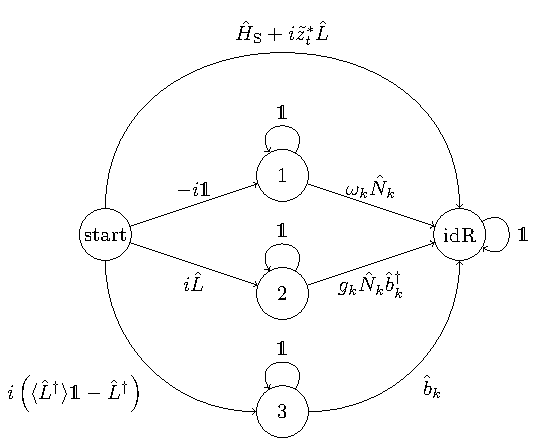
\includegraphics{figures/tikz/state_machine/state_machine.pdf}
    \caption{In this figure the state machine that can be used to generate the MPO (\ref{eq:HOMPS_MPO}) is sketched.
    The state machine can be constructed from equation (\ref{eq:effective_HOPS_Hamiltonian_multiple_bath_modes}). For
    reference on how to use state machines to construct MPOs, see \cite{Motruk:2016}}
    \label{fig:state_machine}
\end{figure}
\subsubsection*{Computing Expectation Values}
The expectation value $\left\langle \hat{L}^\dagger\right\rangle_t$
can be easily computed from the MPS (\ref{eq:HOMPS_MPO}) by setting the index vector $\vb*{n} = \vb*{0}$:
\begin{equation*}
    \left\langle \hat{L}^\dagger\right\rangle_t = \frac{\bra*{\vb*{\Psi}^{(\vb*{0})}_t}\hat{L}^\dagger\ket*{\vb*{\Psi}^{(\vb*{0})}_t}}{\bra*{\vb*{\Psi}^{(\vb*{0})}_t}\ket*{\vb*{\Psi}^{(\vb*{0})}_t}},
\end{equation*}
\begin{equation*}
    \ket*{\vb*{\Psi}^{(\vb*{0})}_t} = \sum_{l,\vb*{i}} A_{i_0,i_1}^{[1],l} A_{i_1,i_2}^{[2],0} A_{i_2,i_3}^{[3],0} \dots A_{i_K,i_0}^{[K+1],0}  \ket*{l}.
\end{equation*}
\subsubsection*{Updating the Memory Terms}
To compute the memory term
\begin{equation*}
    z_\text{memory}^*(t) \coloneqq \int_0^t \alpha^*(t-s) \left\langle L^\dagger\right\rangle_s \text{ds}
    \approx \sum_{k=1}^{K} \int_0^t g_k e^{-\omega_k} \left\langle L^\dagger\right\rangle_s \text{ds}
\end{equation*}
in the "shifted" noise (\ref{eq:memory_term_nonlinear_HOPS}) for $K > 1$ bath modes, we first split it into
$K$ terms
\begin{equation*}
    z_\text{memory}^*(t) = \sum_{k=1}^{K} z_{\text{memory},k}^*(t), \quad z_{\text{memory},k}^*(t) \coloneqq \int_0^t g_k e^{-\omega_k} \left\langle L^\dagger\right\rangle_s \text{ds}.
\end{equation*}
Each of the terms $z_{\text{memory},k}^*(t)$ can then be updated similar to (\ref{eq:memory_update_single_bath_node}).
\section{Benchmarking HOMPS}
\begin{figure}[h]
    \centering
    \begin{tikzpicture}[scale=1]
        \definecolor{color1}{HTML}{deebf4}
        \definecolor{color2}{HTML}{b3d1e7}
        \definecolor{color3}{HTML}{8ab7d9}
        \definecolor{color4}{HTML}{629ccb}
        \definecolor{color5}{HTML}{3182bd}

        \begin{axis}[xlabel=$t$, ylabel=$\left\langle\sigma_z\right\rangle$,
            grid=both, xmin=0, xmax=30, ymin=-.5, ymax=1, no markers, 
            every axis plot/.append style={very thick}]

            \addplot[color = color1]
            table[x=t, y=sigma_z_100, col sep=space]{figures/plots/HOMPS/data/homps_high_T_multiple_realizations.txt};
            \addlegendentry{100 realizations}

            \addplot[color = color3]
            table[x=t, y=sigma_z_1000, col sep=space]{figures/plots/HOMPS/data/homps_high_T_multiple_realizations.txt};
            \addlegendentry{1000 realizations}

            \addplot[color = color5]
            table[x=t, y=sigma_z_10000, col sep=space]{figures/plots/HOMPS/data/homps_high_T_multiple_realizations.txt};
            \addlegendentry{10000 realizations}

        \end{axis}
    \end{tikzpicture} 
    \label{fig:full_runs_HOMPS_high_T} 
    \caption{test}
\end{figure}

\chapter{Conclusion}
\label{chap:Conclusion}
As we have seen, the HOPS method is able to relieably simulate the dynamics of non-Markovian open quantum systems. 
If one wants to use multiple bath modes, the HOMPS method is a good strategy to minimize memory requirements by
compressing the quantum state into Matrix Product form. We discussed two integration methods, RK4 and TDVP2, which are
both viable for solving the HOMPS equations. There are however some additional steps that can be made to further
improve the methods. \\
First, there exists an alternative realization of the non-Markovian stochastic Schrödinger equation \cite{Song:2016},
where, in contrast to (\ref{eq:stochastic_process_condition}), a stochastic process with non-zero correlations 
$\mathbb{E}\left[z_{t}z_{s}\right]\neq0$ is used. This leads to a smaller bath correlation function, reducing the
amplitude of the non-Markovian memory term at high temperatures. For models that need many terms for approximating the 
bath correlation function sufficiently well, this can be a crucial improvement.\\
Second, one has to consider how systems consisting of multiple subsystems, i.e., many-body systems, should be treated in the HOMPS method. Because of the
exponential growth of the Hilbert space, using one tensor for the complete many-body system is inefficient. It is therefore
better to split the system into smaller subsystems and to represent each subsystem by a single tensor. A question that arises
is how to connect the different tensors. One idea is to use an MPS, repeating a structure where each physical tensor is followed
by multiple bath mode tensors, which is done in \cite{Gao:2022}. Alternatively, it could be beneficial to use a tree tensor network \cite{Holzner:2010}
instead. The physical subsystems would then be represented by rank-4 tensors, where two legs are used to connect to the neighbouring subsystems,
one leg is the physical leg, and the last leg is connected to an MPS representing the bath modes.
TDVP2 can be adapted for tree tensor networks \cite{Holzner:2010}. This approach would help to further reduce the
memory requirements for computing the non-Markovian dynamics of open many-body systems.\\
In conclusion, I believe that the HOPS and HOMPS methods are very useful for simulating open quantum systems and will be widely used
for studying new systems and comparing experiments to theory in the future.

\appendix
\chapter{Approximating the BCF of the Spin-Boson model}
\label{app:Approximating_BCF_Spin_Boson}
In this section we derive the coefficients (\ref{eq:expansion_coefficients_debye_BCF_SBM_Matsubara}) and (\ref{eq:expansion_coefficients_debye_BCF_SBM_Pade}) that can be used to approximate the bath correlation function
\begin{equation*}
    \alpha(\tau) = \frac{1}{\pi} \int_0^\infty S(\omega)
    \left[
        \coth\left(\frac{\omega}{2T}\right)\cos(\omega\tau)-i\sin(\omega\tau)
    \right]\text{d}\omega
    = \int_0^\infty I(\omega,\tau)\text{d}\omega
\end{equation*}
with the \textit{Debye spectral density}
\begin{equation*}
    S(\omega) = \eta \frac{\omega\gamma}{\omega^2+\gamma^2}
\end{equation*}
as a sum of exponentials
\begin{equation*}
    \alpha(\tau) \approx \sum_{k=0}^{K-1}g_ke^{-\omega_k\tau}.
\end{equation*}
We first note that the integrand $I(\omega, \tau)$ is symmetric with respect to $\omega$; $\,I(-\omega, \tau) = I(\omega, \tau)$.
Therefore, we can extend the integral over the negative real axis:
\begin{equation*}
    \alpha(\tau) = \frac{1}{2\pi} \int_{-\infty}^\infty S(\omega)
    \left[
        \coth\left(\frac{\omega}{2T}\right)\cos(\omega\tau)-i\sin(\omega\tau)
    \right]\text{d}\omega.
\end{equation*}
Next, we write the sine and cosine in terms of complex exponentials and use the identity $\coth(x) = 2f^\text{Bose}(2x) - 1$
with the \textit{Bose function}
\begin{equation*}
    f^\text{Bose}(x) \coloneqq \frac{1}{1-e^{-x}}
\end{equation*}
to arrive at
\begin{equation}
    \label{eq:transformed_BCF_Bose}
    \alpha(\tau) = \frac{1}{\pi} \int_{-\infty}^\infty S(\omega)
    \left[
        f^\text{Bose}(\omega\beta)-1
    \right]\text{d}\omega.
\end{equation}
In the following, we will derive two different approximations of this integral.

\subsection*{Matsubara frequency summation}
The Matsubara frequency summation uses the residue theorem to turn the integral (\ref{eq:transformed_BCF_Bose}) into an infinite
sum. This sum then has to be truncated to get an approximation with a finite number of terms. The resulting approximation works well at high temperatures,
but converges only slowly at low temperatures.\\
Consider the line integral in Figure \ref{fig:line_integral_matsubara_expansion}. Because of the exponential term
$e^{i\omega\tau}$, the contribution along $L_2$ vanishes as we take the limit $R \rightarrow \infty$. This then leaves us with
\begin{equation*}
    \begin{split}
        \alpha(\tau) &= \frac{1}{\pi} \oint_\xi S(\omega) \left[
            f^\text{Bose}(\omega\beta)-1
        \right]\text{d}\omega = 2i \sum_{\{\omega_j\}}\Res\left(
            S(\omega)e^{-i\omega\tau}\left[
            f^\text{Bose}(\omega\beta)-1
            \right]; \omega_j\right) \\
            &= 2i \sum_{\{\omega_j^\prime\}} \Res\left(
                S(\omega); \omega_j^\prime
            \right) e^{i\omega_j^\prime\tau} \left[ f^\text{Bose}(\omega_j^\prime\beta)-1 \right]
            + 2i\sum_{\{\omega_j^{\prime\prime}\}}\Re\left(
                f^\text{Bose}(\omega\beta); \omega_j^{\prime\prime}
            \right) S(\omega_j^{\prime\prime}) e^{i\omega_j^{\prime\prime}\tau},
    \end{split}
\end{equation*}
where $\omega_j$ are the poles of $S(\omega) \left[f^\text{Bose}(\omega\beta)-1\right]$, $\omega_j^\prime$ the poles of
$S(\omega)$, $\omega_j^{\prime\prime}$ the poles of $f^\text{Bose}(\omega\beta)$, and we have used the residue theorem.
We also assumed that
$\omega_i^\prime \neq \omega_j^{\prime\prime}$ for all $i, j$, which is the case for almost all $\gamma, \beta$.
Next, we need to compute all poles and residues. The Debye spectral density has simple poles at $\omega_j^\prime=\pm i\gamma$,
with residues
\begin{equation*}
    \Residue\left(S(\omega);\pm i\gamma\right) = \lim_{\omega\rightarrow i\gamma}(\omega\mp i\gamma)S(\omega) = \frac{\eta\gamma}{2}.
\end{equation*}
The poles of the Bose function lie on the imaginary axis, $\omega_j^{\prime\prime} = 2\pi in/\beta$ with $n\in\mathbb{Z}$,
and are again simple poles with residues
\begin{equation*}
    \Re\left(
        f^\text{Bose}(\omega\beta); \frac{2\pi in}{\beta}
    \right) = \lim_{\omega \rightarrow 2\pi in/\beta} \frac{(\omega-2\pi in/\beta)}{1-e^{-\omega\beta}} =
    \lim_{x\rightarrow0}\frac{x}{1-e^{-\beta x-2\pi i n}} = \lim_{x\rightarrow0} \frac{1}{\beta e^{-\beta x}} = \frac{1}{\beta},
\end{equation*}
where we substituted $x = \omega - 2\pi i n/\beta$ and used the rule of L'Hopital.\\
With this, we are now equipped to solve the integral:
\begin{equation*}
    \alpha(\tau) = \frac{\eta\gamma}{2} e^{-\gamma\tau}\left[\cot(\gamma\beta)-i\right]e^{-\gamma\tau}
    + \sum_{k=1}^{\infty} \eta\frac{4\pi T^2k\gamma}{4\pi^2T^2k^2-\gamma^2} e^{-2\pi Tk\tau} = \sum_{k=0}^{\infty} g_ke^{-\omega_k\tau}
\end{equation*}
with the coefficients (\ref{eq:expansion_coefficients_debye_BCF_SBM_Matsubara}).
The result is similar to the one obtained in \cite{Qiang:2009} (up to a different normalization).
  
\subsection*{Padé spectrum decomposition}
The Padé spectrum decomposition is a method to approximate the Bose function $f_\text{Bose}(x)$ by a finite sum \cite{Hu:2011}. We will use the Padé approximant
$[N-1/N]$ with $N\equiv K-1$ to rewrite
\begin{equation*}
    \alpha(\tau) \approx \frac{1}{\pi} \int_{-\infty}^{\infty} S(\omega) e^{i\omega\tau}
    \left[
        \frac{1}{\omega\beta}-\frac{1}{2}+\sum_{k=1}^{K-1}\frac{2\tilde{\eta}_k\omega_\beta}{(\omega\beta)^2+\tilde{\xi}_k^2}
    \right]\text{d}\omega,
\end{equation*}
where the derivation of the constants $\tilde{\eta}_k$ and $\tilde{\xi}_k$ can be found in \cite{Hu:2011}.
We can now proceed in a similar way to the Matsubara frequency summation. We will again consider the line integral along
the contour in Figure \ref{fig:line_integral_matsubara_expansion} and use the residue theorem. The poles and residues of the
new terms are
\begin{equation*}
    \Res\left(
        \frac{1}{\omega\beta}; 0
    \right) = \frac{1}{\beta}
\end{equation*} 
and
\begin{equation*}
    \Res\left(
        \frac{2\tilde{\eta}_k\omega\beta}{(\omega\beta)^2+\tilde{\xi}_k^2}; \pm i\frac{\tilde{\xi}_k}{\beta}
    \right) = \frac{\tilde{\eta}_k}{\beta}.
\end{equation*}
A bit of algebra yields the final result
\begin{equation*}
    \alpha(\tau) \approx \eta\gamma\left[
        \frac{1}{\gamma\beta}-\frac{i}{2}-\sum_{k=1}^{K-1}\frac{2\tilde{\eta}_k\gamma\beta}{\tilde{\xi}_k^2-\gamma^2\beta^2}
    \right] e^{-\gamma\tau}
    + \sum_{k=1}^{K-1} \frac{2\tilde{\eta}_k\eta\gamma\tilde{\xi}_k}{\tilde{\xi}_k^2-\gamma^2\beta^2} e^{-\frac{\tilde{\xi}_k}{\beta}\tau}
    = \sum_{k=0}^{K-1}g_ke^{-\omega_k\tau}
\end{equation*}
with the coefficients (\ref{eq:expansion_coefficients_debye_BCF_SBM_Pade}).
\begin{figure}[!ht]
    \centering
    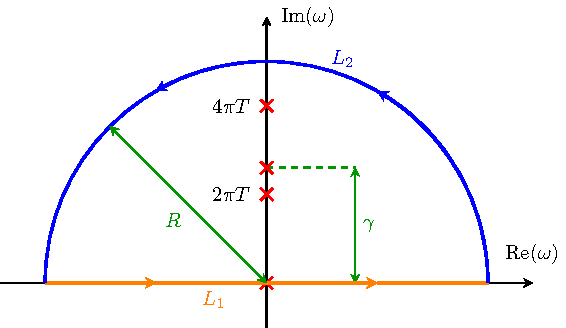
\includegraphics{tikz/matsubara_expansion/matsubara_expansion.pdf}
    \caption[short]{In this figure, the line integral for computing the expansion of the bath correlation function is shown.}
    \label[figure]{fig:line_integral_matsubara_expansion}
\end{figure}
\chapter{Stability of the default and rescaled HOMPS}
\label{app:default_vs_rescaled}
The non-rescaled HOMPS (\ref{eq:HOMPS_MPO}) has numerical stability problems for higher values of $N_\text{trunc}$. To illustrate the problem,
I plot the expectation value $\mathbb{E}\left\lbrack\langle\hat{\sigma}_z\rangle_t\right\rbrack$ of the high temperature spin-boson model in Figure \ref{fig:default_vs_rescaled_sigma_z}, using both
the non-rescaled HOMPS (\ref{eq:HOMPS_MPO}) and the rescaled HOMPS (\ref{eq:HOMPS_MPO_rescaled}). For a better comparison, the stochastic process
was set to $z(t) = 0$ for both methods. A high truncation value of $N_\text{trunc}=40$ was used. One can see that the non-rescaled HOMPS diverges
after a short time and does not produce the correct behaviour. \\
\begin{figure}[!ht]
    \centering
    \begin{tikzpicture}[scale=1, trim axis left, trim axis right]
        \definecolor{color1}{HTML}{4477AA}
        \definecolor{color2}{HTML}{EE6677}
        \def\singleFigureWidth{0.5\textwidth}
        \def\singleFigureHeight{0.309\textwidth}

        \begin{axis}[xlabel=$t$, ylabel=$\mathbb{E}\left\lbrack\langle\hat{\sigma}_z\rangle\right\rbrack$,
            grid=both, xmin=0, xmax=30, ymin=0, ymax=1, no markers, 
            every axis plot/.append style={very thick}, scale only axis, height=\singleFigureHeight, width=\singleFigureWidth,
            legend pos=south west]

            \addplot[color = color1]
            table[x=t, y=sigma_z_default, col sep=space]{figures/plots/Appendix_B/data/rescaled_homps_sigma_z.txt};
            \addlegendentry{non-rescaled HOMPS}

            \addplot[color = color2, dashed]
            table[x=t, y=sigma_z_rescaled, col sep=space]{figures/plots/Appendix_B/data/rescaled_homps_sigma_z.txt};
            \addlegendentry{rescaled HOMPS}

        \end{axis}
    \end{tikzpicture}   
    \caption{The expectation value $\mathbb{E}\left\lbrack\langle\hat{\sigma}_z\rangle\right\rbrack$ is computed for both the non-rescaled and the
    rescaled HOMPS. I use the high temperature spin-boson model with the same parameters as in Figure \ref{fig:homps_high_T_full_runs}, but only compute a single realization whithout noise ($z(t) = 0$).
    One can see that the non-rescaled version of HOMPS is unstable, diverging after a short time.}
    \label{fig:default_vs_rescaled_sigma_z} 
\end{figure}
\newline
\noindent The reason for this instability could be the fact that different auxillary states have vastly different magnitudes in the non-rescaled
version of HOMPS. In Figure \ref{fig:default_vs_rescaled_magnitudes}, I plot the magnitudes of the different auxillary states of both the non-rescaled and rescaled HOMPS against 
time. One can see that the non-rescaled version produces magnitudes that differ by up to 15 orders of magnitudes, whereas in the rescaled
version they differ only up to 7 orders of magnitude. In the HOMPS method addition of tensors is performed, which could lead to cancellation,
a well-known limitation of floating point arithmetic. The rescaling "normalizes" the auxillary states and increases numerical stability. 
\begin{figure}[!ht]
    \def\doubleFigureWidth{5cm}
    \def\doubleFigureHeight{4.635cm}
    \centering
    \begin{subfigure}[b]{0.34\textwidth}
        \begin{tikzpicture}[scale=1]
            \begin{axis}[xlabel=$t$, ylabel=$||\Psi^{(n)}_t||$,
                grid=both, xmin=0, xmax=30, ymin=1e-16, ymax=1, no markers, 
                every axis plot/.append style={very thick}, 
                scale only axis, height=\doubleFigureHeight, width=\doubleFigureWidth, ymode=log, title=Not Rescaled,
                point meta min=1, point meta max=40,
                cycle list={[samples of colormap={40 of colormap/Blues-3}]}]

                \foreach \x in {0,...,39}{
                    \addplot table [col sep=space, x=t, y=\x] {figures/plots/Appendix_B/data/auxillary_magnitudes_default.txt};
                }


            \end{axis}
        \end{tikzpicture}
    \end{subfigure}
    \centering
    \begin{subfigure}[b]{0.64\textwidth}
        \centering
        \begin{tikzpicture}
            \begin{axis}[xlabel=$t$, yticklabels={,,}, legend pos=south east,
                grid=both, xmin=0, xmax=30, ymin=1e-16, ymax=1, no markers, 
                every axis plot/.append style={very thick}, 
                scale only axis, height=\doubleFigureHeight, width=\doubleFigureWidth, legend pos=north east, ymode=log, title = Rescaled,
                cycle list={[samples of colormap={40 of colormap/Blues-3}]},
                colorbar, colormap/Blues-3, 
                colorbar style={
                    title=$n$,
                    yticklabels={0,10,20,30,40},
                    ytick = {0,0.25,0.5,0.75,1},
                },
                point meta max = 1,
                point meta min = 0]

                \foreach \x in {0,...,39}{
                    \addplot table [col sep=space, x=t, y=\x] {figures/plots/Appendix_B/data/auxillary_magnitudes_rescaled.txt};
                }

            \end{axis}
        \end{tikzpicture}
    \end{subfigure}
    \caption{In this figure, the magnitudes of different HOMPS auxillary states $\Psi^{(n)}_t$ are plotted against $t$. I use the high temperature
    spin-boson model with the same parameters as in Figure \ref{fig:homps_high_T_full_runs}, but only compute a single realization whithout noise ($z(t) = 0$).
    One can see that the magnitudes of different auxillary states take on vastly more widespread values when using the non-rescaled version of
    HOMPS than when using the rescaled version.}
    \label{fig:default_vs_rescaled_magnitudes} 
\end{figure}

\backmatter{}

\printbibliography{} % print bibliography
\end{refsection}
\begin{refsection}
\nocite{Website:ColorBrewer}
\nocite{Website:ColorBlind}
\printbibliography[heading=subbibliography, title={Resources for Plotting}]
\end{refsection}

\newpage
\thispagestyle{empty}
\noindent\textbf{\large Benchmarking a Tensor Network Algorithm for the HOPS-Method to Simulate Open non-Markovian Quantum Sytems}
\vspace*{0.5cm}
\par\noindent Benjamin Sappler

\end{document}
